\documentclass[%
  aspectratio=169,
  9pt,
  USenglish,
  titlegraphic, % store custom image to .images/titlegraphic
  affiliationintitlepagehead,
  %progressbar,
  affiliation,
]{beamer}

\usetheme{TUM}

\usepackage{tikz}  
\usepackage{tikz-3dplot} 
\usepackage{graphicx}
\usepackage{media9}
\usetikzlibrary{positioning}

\usepackage{amsmath}
\usepackage{booktabs}

% change the camera position
\tdplotsetmaincoords{45}{135}



\usepackage{animate}

\usepackage{pgfmath}
\newcommand\randmin{}
\newcommand\randmax{}
\newcommand\randmultof{}
\newcommand\setrand[4]%
{\def\randmin{#1}%
	\def\randmax{#2}%
	\def\randmultof{#3}%
	\pgfmathsetseed{#4}%
}
\newcommand\nextrand
{\pgfmathparse{int(int((rnd*(\randmax-\randmin+1)+\randmin)/\randmultof)*\randmultof)}%
	\xdef\thisrand{\pgfmathresult}%
}

%\usepackage[backend=biber]{biblatex}
%\addbibresource{bib/references.bib}

\newcommand{\wave}{
	\begin{tikzpicture}[xscale=.05,yscale=.2]
	\draw[-,fill=white] plot[domain=0:10*pi,smooth] (\x,{sin(\x r)});
	\end{tikzpicture}
}


\newcommand{\domain}[4]{
	%% spatial,spectral,temporal
	\draw[fill=#4, opacity=.2] (#1,0,0) -- (0,#2,0) -- (0,0,#3) -- (#1,0,0);
}


\newcommand{\radarwave}{
	\begin{tikzpicture}[xscale=.1,yscale=.2]
	\draw[-,fill=white] plot[domain=0:5*pi,smooth] (\x,{sin(\x r)});
	\end{tikzpicture}
}


\newcommand{\earth}{
	\begin{tikzpicture}[baseline=-.25em, inner sep=0]
	\node{
\includegraphics[width=8mm]{images/icons/earth}};
	\end{tikzpicture}
}

\newcommand{\sat}{
	\begin{tikzpicture}[baseline=-.25em, inner sep=0]
	\node[rotate=270,anchor=center]{
\includegraphics[width=8mm]{images/icons/sat2}};
	\end{tikzpicture}
}


\usepackage[capitalize]{cleveref}
\usepackage[square,sort,comma,numbers]{natbib}

%% this hack seems to be nececessary due to incompatibilities of cvpr template and tikz... -> https://tex.stackexchange.com/questions/398223/tikz-gives-error-command-everyshipouthook-already-defined
%\makeatletter
%\@namedef{ver@everyshi.sty}{}
%\makeatother
%% hackend

\usepackage{tikz}
\usepackage{pgfplots}
\usetikzlibrary{positioning, calc,arrows,arrows.meta, fit}
%\usetikzlibrary{arrows.meta,calc,decorations.markings,math,arrows.meta}
\usepgfplotslibrary{groupplots}
\usepgfplotslibrary{fillbetween}
\usepgfplotslibrary{statistics} % provides boxplots
\usepackage{xfrac}

\newcommand{\tp}{tp}
\newcommand{\tn}{tn}
\newcommand{\fp}{fp}
\newcommand{\fn}{fn}


\usepackage{tumcolors}
\usepackage{tummath}
\newcommand{\yhat}{\hat{\V{y}}}
\newcommand{\ycorrect}{\hat{y}^+}
\newcommand{\thetadelta}{\V{\Theta}_\delta}
\newcommand{\biasdelta}{b_\delta}
\newcommand{\biasclass}{\V{b}_\text{c}}
\newcommand{\thetaclass}{\V{\Theta}_\text{c}}
\newcommand{\thetafeat}{\V{\Theta}_\text{feat}}
\newcommand{\fclass}{f_\text{c}}
\newcommand{\fdelta}{f_\delta}
\newcommand{\ffeat}{f_\text{feat}}
\newcommand{\f}{f}

\newcommand{\rvtime}{T_c} 
\newcommand{\xuptot}{\M{X}_{\rightarrow t}} 
\newcommand{\deltauptot}{\delta_{\rightarrow t}} 
\newcommand{\tstop}{\ensuremath{t_\text{stop}}}
\newcommand{\meantstop}{\ensuremath{\bar{t}_\text{stop}}}
\usepackage[super]{nth}
\usepackage{mathtools}

\definecolor{evalcolor}{HTML}{3F3F3F}
\definecolor{traincolor}{HTML}{B98951}
\definecolor{validcolor}{HTML}{3F4BBE}

\definecolor{fdlcolor}{HTML}{142737}


\colorlet{colortrain}{tumblue}
\colorlet{colorinfer}{tumblack}

\colorlet{earlinesscolor}{tumblue}
\colorlet{accuracycolor}{tumorange}

\colorlet{stdcolor}{tumbluelight}
\colorlet{mediancolor}{tumorange}
\colorlet{meancolor}{tumblue}

\colorlet{b1color}{tumdiagramaubergine}
\colorlet{b2color}{tumdiagramnavyblue}
\colorlet{b3color}{tumdiagramturquoise}
\colorlet{b4color}{tumdiagramgreen}
\colorlet{b5color}{tumdiagramlimegreen}
\colorlet{b6color}{tumdiagramyellow}
\colorlet{b7color}{tumdiagramsand}
\colorlet{b8color}{tumdiagramredorange}
\colorlet{b8Acolor}{tumdiagramred}
\colorlet{b9color}{tumblack}
\colorlet{b10color}{tumblue}
\colorlet{b11color}{tumdiagramdarkred}
\colorlet{b12color}{tumorange}

% atmospheric bands
\colorlet{b1color}{tumblack}%tumdiagramaubergine
\colorlet{b9color}{tumblack}%tumblack
\colorlet{b10color}{tumblack}%tumblue

%visisble bands
\colorlet{b2color}{tumblue}%tumdiagramnavyblue
\colorlet{b3color}{tumblue}%tumdiagramturquoise
\colorlet{b4color}{tumblue}%tumdiagramgreen

% near infrared bands
\colorlet{b5color}{tumdiagramred}%tumdiagramlimegreen
\colorlet{b6color}{tumdiagramred}%tumdiagramyellow
\colorlet{b7color}{tumdiagramred}%tumdiagramsand
\colorlet{b8color}{tumdiagramred}%tumdiagramredorange
\colorlet{b8Acolor}{tumdiagramred}%tumdiagramred

% SWIR bands
\colorlet{b11color}{tumorange}%tumdiagramdarkred
\colorlet{b12color}{tumorange}%tumorange

\colorlet{epsilon0color}{tumorange}
\colorlet{epsilon1color}{tumblue}
\colorlet{epsilon10color}{tumblack}

\colorlet{gridcolor}{tumblue}
\colorlet{activationcolor}{tumorange}

\colorlet{meadowcolor}{tumbluemedium}
\colorlet{wbarleycolor}{tumbluedark}
\colorlet{corncolor}{tumorange}
\colorlet{wheatcolor}{tumgreen}
\colorlet{sbarleycolor}{tumdiagramred}
\colorlet{clovercolor}{tumdiagramturquoise}
\colorlet{triticalecolor}{tumdiagramsand}

\tikzstyle{rnn}=[draw,circle, inner sep=.1em]
\tikzstyle{norm}=[rounded corners,draw]
\tikzstyle{annot}=[rounded corners, fill=tumblue!20]
\tikzstyle{infer}=[-stealth, shorten >=.0em, shorten <=.0em, colorinfer]
\tikzstyle{loss}=[fill=tumblue!10, rounded corners, font=\small]
\tikzstyle{grad}=[colortrain]

\newcommand{\ptoffset}{\varepsilon}

\tikzstyle{test} = [thick]
\tikzstyle{train} = [thin, dotted]

\usepackage[inline]{enumitem}
\setenumerate{label=(\roman*),itemsep=3pt,topsep=3pt}

\setlength{\belowcaptionskip}{-10pt}


\colorlet{traincolor}{tumbluelight}
\colorlet{validcolor}{tumbluedark}
\colorlet{evalcolor}{tumorange}

\colorlet{forwardcolor}{tumblue}
\colorlet{backwardcolor}{tumorange}

% defaultvalue -> might be replaced later
\colorlet{tensorcolor}{forwardcolor}

\colorlet{classcolor}{tumivory}
\colorlet{encodercolor}{tumblue}
\colorlet{encodercolor}{tumblue}
\colorlet{colorblue}{tumblue}
\colorlet{colororange}{tumorange}

\colorlet{colorclassone}{tumblue}
\colorlet{colorclasstwo}{tumblack}
\colorlet{colorclassthree}{tumorange}
\colorlet{colorclassfour}{tumgray}

\colorlet{frh01color}{tumgray}
\colorlet{frh02color}{tumorange}
\colorlet{frh03color}{tumblue}
\colorlet{frh04color}{tumblack}



%\usepackage{media9}

% notation
\newcommand{\MWeight}{\ensuremath{\M{W}}}
\newcommand{\VBias}{\ensuremath{\V{b}}}
\newcommand{\VInput}{\DataVec}
\newcommand{\VHidden}{\ensuremath{\V{h}}}
\newcommand{\FActivation}{\ensuremath{\sigma}}
\newcommand{\VCellState}{\ensuremath{\V{c}}}
\newcommand{\VForgetGate}{\ensuremath{\V{f}}}
\newcommand{\VModulationGate}{\ensuremath{\V{j}}}
\newcommand{\VInputGate}{\ensuremath{\V{i}}}
\newcommand{\VOutputGate}{\ensuremath{\V{o}}}



\newcommand{\VResetGate}{\ensuremath{\V{r}}}
\newcommand{\VUpdateGate}{\ensuremath{\V{u}}}


%\usepackage{titlesec}
%\titlespacing{\section}{0pt}{10pt}{3pt}


\usetikzlibrary{3d}
\tikzstyle{perspective3d}=[
x={(0.5cm,0.5cm)}, y={(1cm,0cm)}, z={(0cm,1cm)}]


\usetikzlibrary{spy}

\usetikzlibrary{external,pgfplots.dateplot}

\usepackage[eulergreek]{sansmath}
\pgfplotsset{
	y tick label style={/pgf/number format/.cd,%
		scaled y ticks = false,
		set thousands separator={},
		fixed},
	x tick label style={/pgf/number format/.cd,%
		scaled x ticks = false,
		set decimal separator={,},
		fixed},
	tick label style = {font=\scriptsize\sansmath\sffamily},
	every axis label = {
		font=\scriptsize\sansmath\sffamily},
	every axis/.append style={
		axis lines=left, 
		enlargelimits, 
		thick},
	legend style = {font=\scriptsize\sansmath\sffamily, draw=none, rounded corners=0, fill opacity=.5, text opacity=1},
	label style = {font=\scriptsize\sansmath\sffamily},
	grid style={line width=.1pt, draw=gray!10},
	major grid style={line width=.2pt,draw=tumgraylight},
}

%\let\tempone\itemize
%\let\temptwo\enditemize
%\renewenvironment{itemize}{\tempone\addtolength{\itemsep}{-.5\baselineskip}}{\temptwo}

\tikzstyle{circ} = [circle, draw=white, fill=tumblue, inner sep=1pt]
\newcommand{\fcn}{
	\begin{tikzpicture}[scale=0.2, rotate=0, baseline=-.25em, inner sep=1pt]
	\node[circ](a0) at (0,-1){};
	\node[circ](a1) at (0,0){};
	\node[circ](a2) at (0,1){};
	
	\node[circ](b0) at (1,-0.5){};
	\node[circ](b1) at (1,0.5){};
	
	\draw[-] (a0) -- (b0);
	\draw[-] (a1) -- (b0);
	\draw[-] (a2) -- (b0);
	
	\draw[-] (a0) -- (b1);
	\draw[-] (a1) -- (b1);
	\draw[-] (a2) -- (b1);
	
	\end{tikzpicture}
}

\newcommand{\lfcn}[1]{
	\begin{tikzpicture}[scale=#1, rotate=0, baseline=-.25em, inner sep=1pt]
	\node[circle, draw=white, fill=tumblue, inner sep=3](a0) at (0,-1){};
	\node[circle, draw=white, fill=tumblue,  inner sep=3](a1) at (0,0){};
	\node[circle, draw=white, fill=tumblue,  inner sep=3](a2) at (0,1){};
	
	\node[circle, draw=white, fill=tumblue,  inner sep=3](b0) at (1,-0.5){};
	\node[circle, draw=white, fill=tumblue,  inner sep=3](b1) at (1,0.5){};
	
	\draw[-] (a0) -- (b0);
	\draw[-] (a1) -- (b0);
	\draw[-] (a2) -- (b0);
	
	\draw[-] (a0) -- (b1);
	\draw[-] (a1) -- (b1);
	\draw[-] (a2) -- (b1);
	
	\end{tikzpicture}
}

\newcommand{\hidden}[1]{
	\begin{tikzpicture}[scale=.1, baseline=-.25em]	
	%\draw[step=1.0,black,thin] (0,0) grid (#1,1);
	\foreach \i in {1,...,#1}{
		\node[circle, draw=white, fill=tumbluelight, inner sep=1pt] at (\i,0){};
	}
	\end{tikzpicture}
}

\newcommand{\drawvector}[1]{
	\begin{tikzpicture}[scale=.1, baseline=-.25em]	
	%\draw[step=1.0,black,thin] (0,0) grid (#1,1);
	\foreach \i in {1,...,#1}{
		\node[circ] at (\i,0){};
	}
	\end{tikzpicture}
}


\usetikzlibrary{external}
\tikzexternalize[prefix=tikz/]
\tikzexternalize
\tikzexternaldisable

\usepackage{tummath}

\setbeamertemplate{blocks}[rounded][shadow=false]

%	\end{itemize}
%	
%	Research Scope 
%	\begin{itemize}
%		\item Imbalance of Raster and Label Data
%		\item Analogies to NLP
%		\item Sequence modeling
%	\end{itemize}
%		
%	Research Projects
%	\begin{itemize}
%		\item Crop Classification with Multi-temporal Land Cover Classification
%		\item Early Classificaiton of Time Series
%	\end{itemize}
%		
%		
%\end{frame}


\title{BreizhCrops}
\subtitle{A Satellite Time Series Dataset for Crop Type Identification}
\author[M. Rußwurm, S. Lefèvre, M.Körner]{Marc Rußwurm,\footnotemark[1] Sébastien Lefèvre,\footnotemark[2] Marco Körner\footnotemark[1]}
\institute[TUM]{\footnotemark[1]Technical University of Munich, Remote Sensing Technology,  \\
	\footnotemark[2] IRISA-Obelix University of South Brittany}
\date{\today, Time Series Workshop ICML 2019}

\begin{document}

\begin{frame}[t]
\titlepage
\end{frame}


\begin{frame}
\frametitle{System Earth}

\begin{columns}
	
	\column{.5\textwidth}
	
	{
		%		The Earth is a complex system.
		%		Only some components is observable by 
		%		\begin{itemize}
		%			\item satellite-based or
		%			\item in-situ observations
		%		\end{itemize}
		%		
		
		%	\begin{equation*}\V{y} = f({\M{X}})\end{equation*}
		%	partially observe the complex system Earth
		\textbf{Partially measuring} System Earth
		{\Huge
			\begin{equation*}
			\M{X} = \sat\left({\earth}\right)
			\end{equation*}
		}
		
		\vspace{1em}
		\textbf{knowledge extraction} through pattern recognition and machine learning
		
		{\Huge\begin{equation*}\V{?} = f({\M{X}})\end{equation*}}
	}
	
	\column{.5\textwidth}
	
	\begin{tikzpicture}[xscale=3, yscale=2]
	\node(earth) at (0,0) {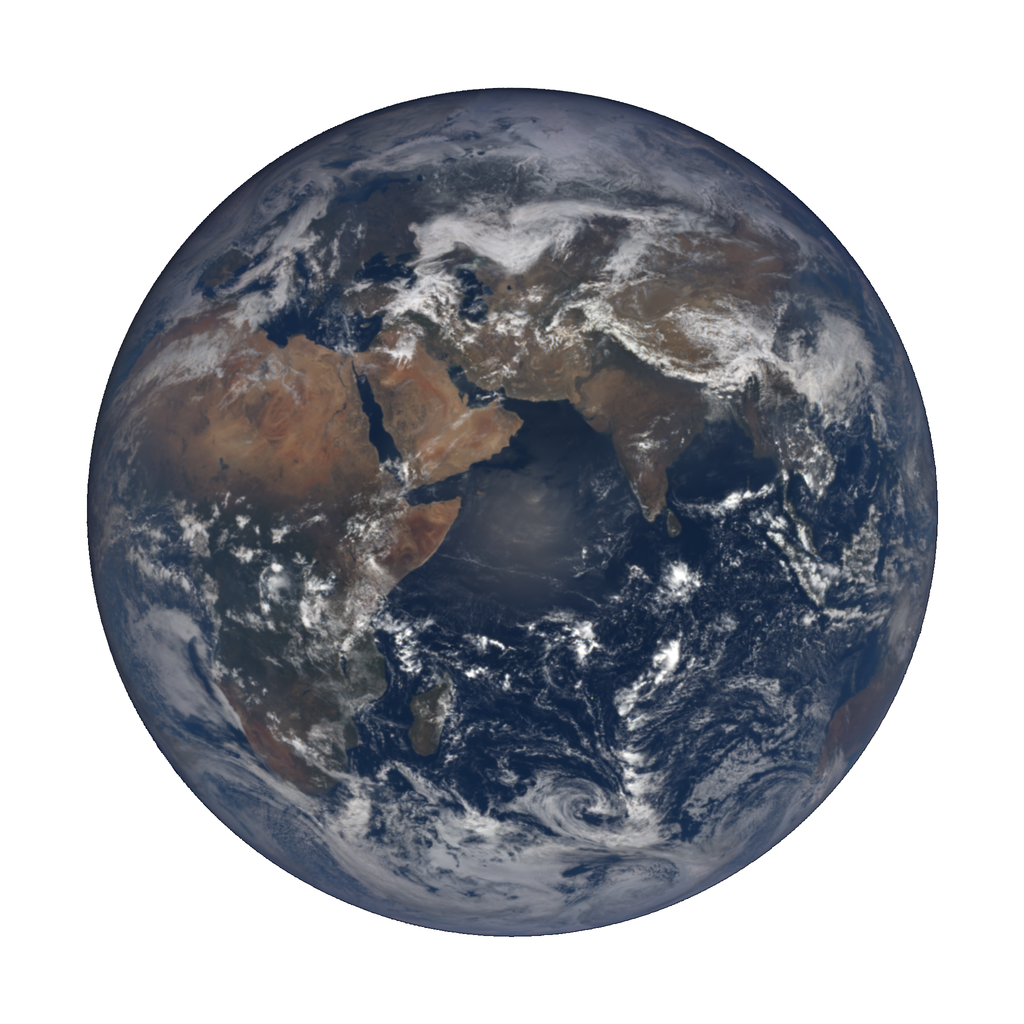
\includegraphics[width=7cm]{images/epicw1}};	
	
	\end{tikzpicture}
	
	
\end{columns}
\end{frame}


%
\begin{frame}
\frametitle{Passive Optical Sensors}
\begin{columns}
	\column{.5\textwidth}
	
	
	\begin{itemize}[itemsep=.5em]
		\item<1-> Sensor measures \textbf{Digital Numbers} $\text{DN}(\lambda)$ for each band wavelength $\lambda$. 
		\item<2-> \textbf{Digital Numbers} are normalized to \textbf{Radiance} 
		$L(\lambda), \left[\frac{W}{\text{sr}m^1}\right]$ by gain and offset calibration.
		\item<4-> Radiance is normalized to \textbf{top-of-atmosphere reflectance} $\rho(\lambda)$
		\item<4-> \textbf{Bottom-of-atmosphere reflectances} are reconstructed using a functional model of the atmosphere.
	\end{itemize}
	
	%	Radiance $R_\lambda$ from measured Digital Numbers via calibrated gain $\alpha$ and offset $\beta$
	%	\begin{equation*}
	%		L_\lambda = \alpha \text{DN}_\lambda + \beta, \left[\frac{W}{\text{sr}m^1}\right]
	%	\end{equation*}
	%	
	%	top-of-atmosphere reflectance $\rho_\lambda$ as normalized Radiance $R_\lambda$ with solar 
	%	\begin{equation*}
	%	\rho_\lambda = \frac{L_\lambda}{\cos(\varphi_\text{sun})}
	%	\frac{
	%		\pi d^2
	%	}
	%	{
	%		E_\text{sun}(\lambda)
	%	}
	%	\end{equation*}
	%	
	%	\vspace{1em}
	%	
	%	\begin{itemize}
	%		\item measured radiance $L(\lambda)$
	%		\item solar irradiance $E_\text{sun}(\lambda)$
	%		\item solar zenith angle $\varphi_\text{sun}$
	%		\item squared Earth-Sun distance $d$ in AU
	%	\end{itemize}
	
	
	\column{.5\textwidth}
	
	
	\begin{tikzpicture}
	
	
	%	\draw [black,dotted, fill=tumbluelight,domain=110:70] plot ({13*cos(\x)}, {13*sin(\x)-12.8});
	\draw [fill=tumivory,domain=110:70] plot ({10*cos(\x)}, {10*sin(\x)-10});
	%	\draw [fill=tumbluelight,domain=110:70] plot ({12*cos(\x)}f, {12*sin(\x)-10});
	
	
	\node(sun) at (-2,2) {
\includegraphics[width=10mm]{images/icons/sun}};
	\node[rotate=130,anchor=center](sat) at (2,2) {
\includegraphics[width=10mm]{images/icons/sat2}};
	
	\node(px) at ({10*cos(90)}, {10*sin(90)-10.1}){
		\begin{tikzpicture}[xscale=.5,yscale=.25]
		\draw[fill=tumbluelight] (0,0) -- (1,0) -- (2,1) -- (1,1) -- (0,0);
		\end{tikzpicture}
		%
\includegraphics[width=5mm]{images/icons/house}
	};
	
	\draw[-stealth] (sun) -- node[midway,sloped]{\wave} (px);
	\draw[-stealth] (px) -- node[midway,sloped]{\wave} (sat);
	
	\visible<3->{\draw[-stealth] (sun) -- node[midway,sloped]{\wave} (sat);
		\draw[draw=tumgray] (px) -- node[at end,left]{$\varphi_\text{sun}$} ++(0,1.4); 
		\draw [draw=tumgray, domain=130:90] plot ({1*cos(\x)}, {1*sin(\x)});
	}
	
	\node[above=.5em of sun]{$E_\text{sun}(\lambda)$};
	\visible<1>{\node[above=4em of sat]{$DN(\lambda)$};}
	\visible<2>{\node[above=4em of sat]{$L(\lambda)$};}
	\visible<3>{\node[above=4em of sat]{$\rho_\text{toa}(\lambda)$};}
	\visible<4>{\node[above=4em of sat]{$\rho_\text{boa}(\lambda)$};}
	
	%		\draw[red] (0,0) sin (1,2);
	
\end{tikzpicture}

\end{columns}

\end{frame}

\newcommand{\rastergrid}{
\begin{tikzpicture}
% each layer
\begin{scope}[scale=2]

% raster size
\def\d{0.7}		

% distance layer
\def\s{\d*5}

\foreach \i in {1,...,6}
{		
\begin{scope}[
yshift=\s*\i,every node/.append style={
	yslant=0.5,xslant=-1},yslant=0.5,xslant=-1
]
%\draw[step=3.33mm] (0,0) grid (1,1);
%\fill[black,fill opacity=.9] (0.333,0.333) rectangle (0.333,0.333);    	    	  

\foreach \row in {0,...,2}{
	\foreach \col in {0,...,2}{
		\draw[tumblack, fill=tumblue!\pdfuniformdeviate 40,fill opacity=1,rounded corners=1] (\col*\d/3,\row*\d/3) rectangle (\col*\d/3+\d/3, \row*\d/3+\d/3);
		%                 \draw[black, fill=black!\pdfuniformdeviate 40,fill opacity=1,rounded corners=1] (\col*\d/3,\row*\d/3) rectangle (\col*\d/3+\d/3, \row*\d/3+\d/3);
	}
}

%\draw[step=3.33mm] (0,0) grid (1,1);
%\fill[white,fill opacity=.9] (0,0) rectangle (1,1);
\end{scope}
}
\end{scope}
\end{tikzpicture}
}


%\begin{frame}
%\frametitle{Spectral Band}
%\end{frame}


\newcommand{\myvec}[1]{\ensuremath{\begin{pmatrix}#1\end{pmatrix}}}
\begin{frame}
\frametitle{Spatial and Temporal Discretization}

\begin{columns}
\column{.5\textwidth}

{
\begin{equation*}
\M{X} = \myvec{\rho_{\lambda_1} \\ \rho_{\lambda_2} \\ \dots \\ \rho_{\lambda_n}}
\end{equation*}
}



Spectral reflectance of \textbf{spectral bands} disctretized on a \textbf{spatial grid}. Each grid cell is georeferenced by its Longitude $\Lambda$ and Latitude $\Phi$.
Acquisitions in regular \textbf{temporal intervals}.

\column{.5\textwidth}



\begin{tikzpicture}

%	\node(a){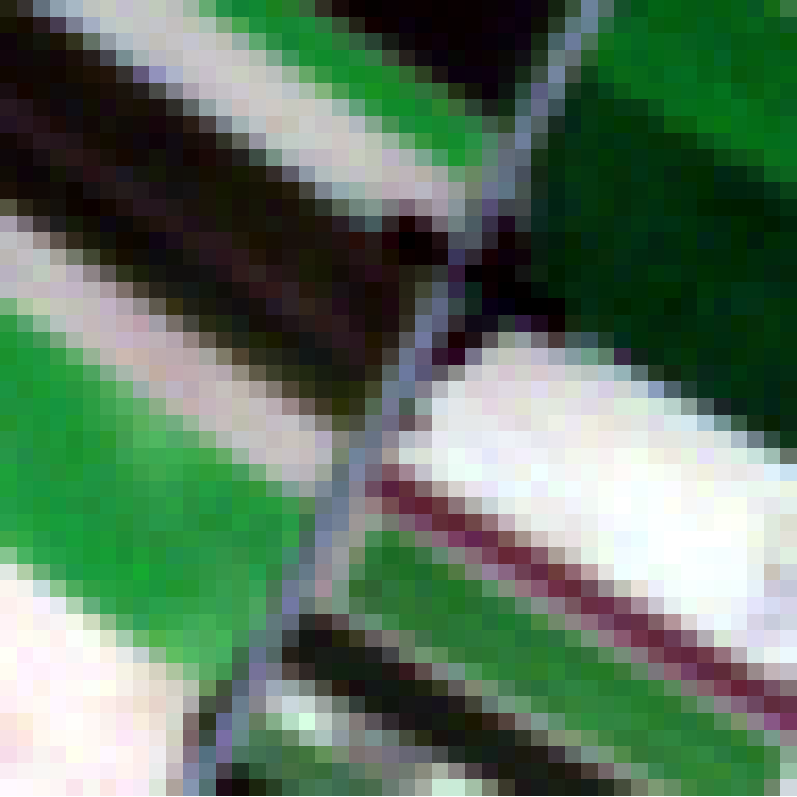
\includegraphics[width=3cm]{images/s2grid/1}};

%	\draw[step=1cm,gray,very thin] (-2,-2) grid (6,6);


\draw [fill=tumivory,domain=110:70] plot ({11*cos(\x)}, {11*sin(\x)-8.5});

\begin{scope}[scale=1]

% raster size
\def\d{1}		

% distance layer
\def\s{\d*50}

\node at (-1.7,2.4){$t_{i-1}$};
\node at (-1.7,4.2){$t_i$};
\node at (-1.7,6){$t_{i-1}$};

\node at (1,1.9){$\Lambda$};
\node at (-1,1.9){$\Phi$};

%		\draw[step=1.0,black,thin] (-2,0) grid (2,5);


\foreach \i in {1,...,3}
{		

\begin{scope}[
yshift=\s*\i,every node/.append style={
	yslant=0.5,xslant=-1},yslant=0.5,xslant=-1,scale=0.35
]
%\draw[step=3.33mm] (0,0) grid (1,1);
%\fill[black,fill opacity=.9] (0.333,0.333) rectangle (0.333,0.333);    	    	  



\foreach \row in {0,...,3}{
	\foreach \col in {0,...,3}{
		\draw[tumblack, fill=tumblue!\pdfuniformdeviate 40,fill opacity=1,rounded corners=1] (\col,\row) rectangle (\col+1, \row+1);
		
		\node[font=\tiny, text=tumblue] at (\col + 0.5,\row + 0.5) {$\V{x}$};
		
		%                 \draw[black, fill=black!\pdfuniformdeviate 40,fill opacity=1,rounded corners=1] (\col*\d/3,\row*\d/3) rectangle (\col*\d/3+\d/3, \row*\d/3+\d/3);
	}
}

%\draw[step=3.33mm] (0,0) grid (1,1);
%\fill[white,fill opacity=.9] (0,0) rectangle (1,1);
\end{scope}
}
\end{scope}



\end{tikzpicture}

\end{columns}


\end{frame}

\begin{frame}
\frametitle{Multi-temporal Vegetation Monitoring}

\begin{columns}
	\column{.5\textwidth}
	
	\begin{tikzpicture}
	\node[] at (0,0){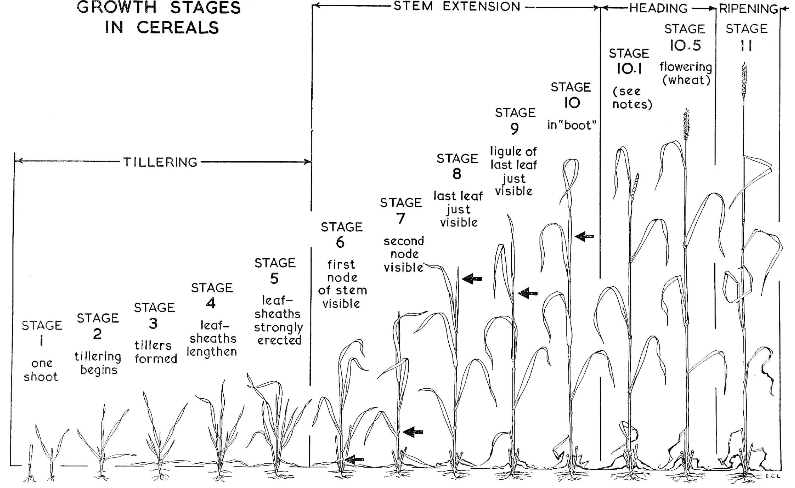
\includegraphics[width=\textwidth]{images/Large1954_cerial_growth_stages}};
	
	%		\draw[step=1.0,black,thin, fill=none] (-2,-2) grid (2,2);
	
	\visible<-1>{\draw [fill=white, draw=none, opacity=0.8] (-0.8,-3) rectangle (2,2.5);}
	\visible<-2>{\draw [fill=white, draw=none, opacity=0.8] (2,-3) rectangle (5,2.5);}
	
	\visible<1>{\node[rotate=190] at (-2.5,1.5){
\includegraphics[width=15mm]{images/icons/sat2}};}
	\visible<2>{\node[rotate=225] at (-2.5,1.5){
\includegraphics[width=15mm]{images/icons/sat2}};}
	\visible<3->{\node[rotate=260] at (-2.5,1.5){
\includegraphics[width=15mm]{images/icons/sat2}};}
	
	
	\visible<4->{\node at (-1.5,1.4) {
\includegraphics[width=10mm]{images/cloud}};
	}
	
	\end{tikzpicture}
	
	\column{.5\textwidth}
	
	{\Large
		\only<1>{
			\begin{equation*}
			\V{y} = f_\text{phenology}(\V{X}_t)
			\end{equation*}
		}
		\only<2>{
			\begin{equation*}
			\V{y} = f_\text{phenology}(\V{X}_t,\V{X}_{t+1})
			\end{equation*}
		}
		\only<3>{
			\begin{equation*}
			\V{y} = f_\text{phenology}(\V{X}_t,\V{X}_{t+1},\V{X}_{t+2})
			\end{equation*}
		}
	}
	
	
	\vspace{2em}
	
	
	\visible<1->{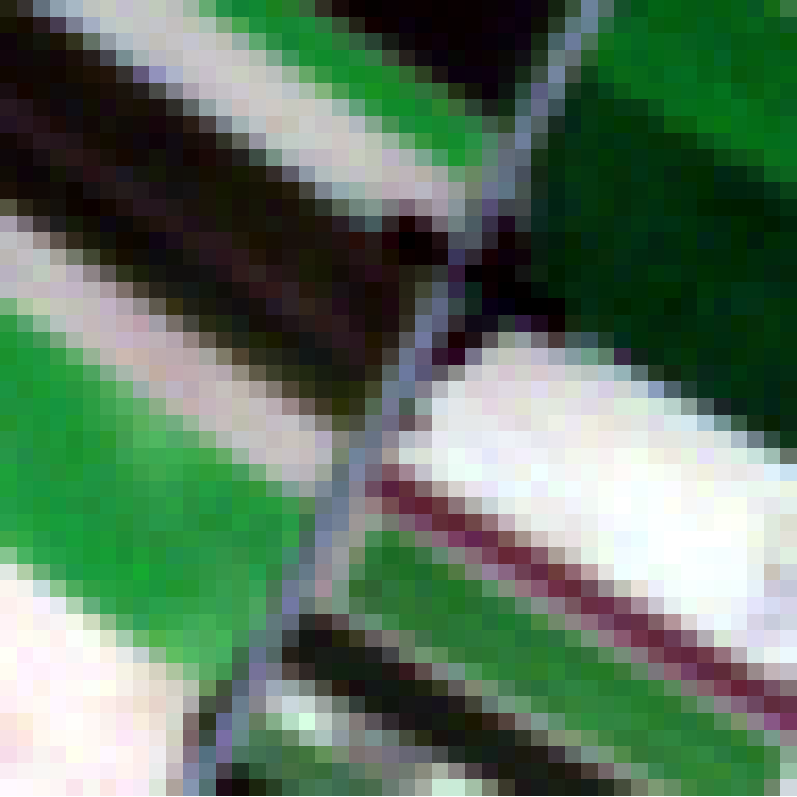
\includegraphics[width=.22\textwidth]{images/s2grid/1}}
	\visible<2->{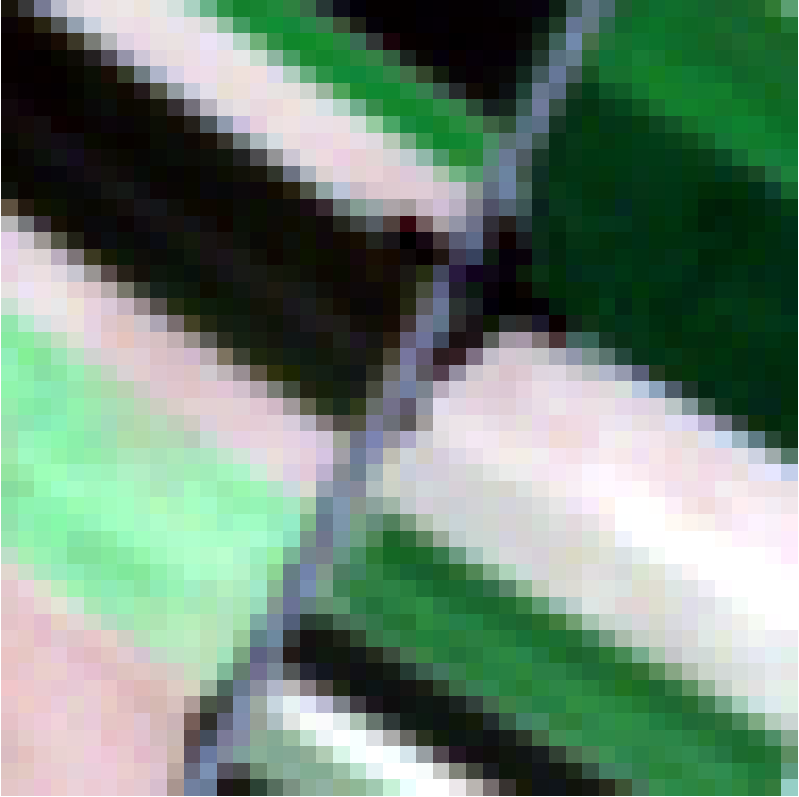
\includegraphics[width=.22\textwidth]{images/s2grid/2}}
	\visible<3->{
\includegraphics[width=.22\textwidth]{images/s2grid/3}}
	\visible<4->{
\includegraphics[width=.22\textwidth]{images/s2grid/4}}
	
	\vspace{1em}
	
	{\small 
		Large, E. C. (1954). Growth stages in cereals illustration of the Feekes scale. Plant pathology, 3(4), 128-129.
	}
	
	
\end{columns}
\end{frame}


\begin{frame}
\frametitle{BreizhCrops Dataset (available by next week!)}

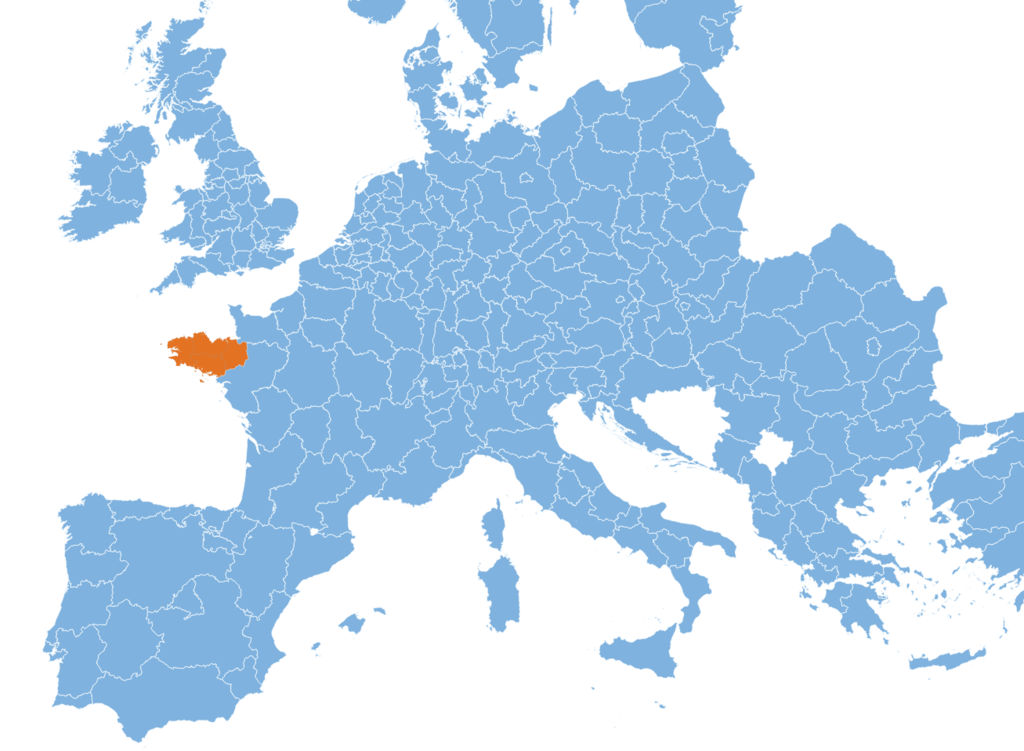
\includegraphics[width=3cm]{images/map/europe}
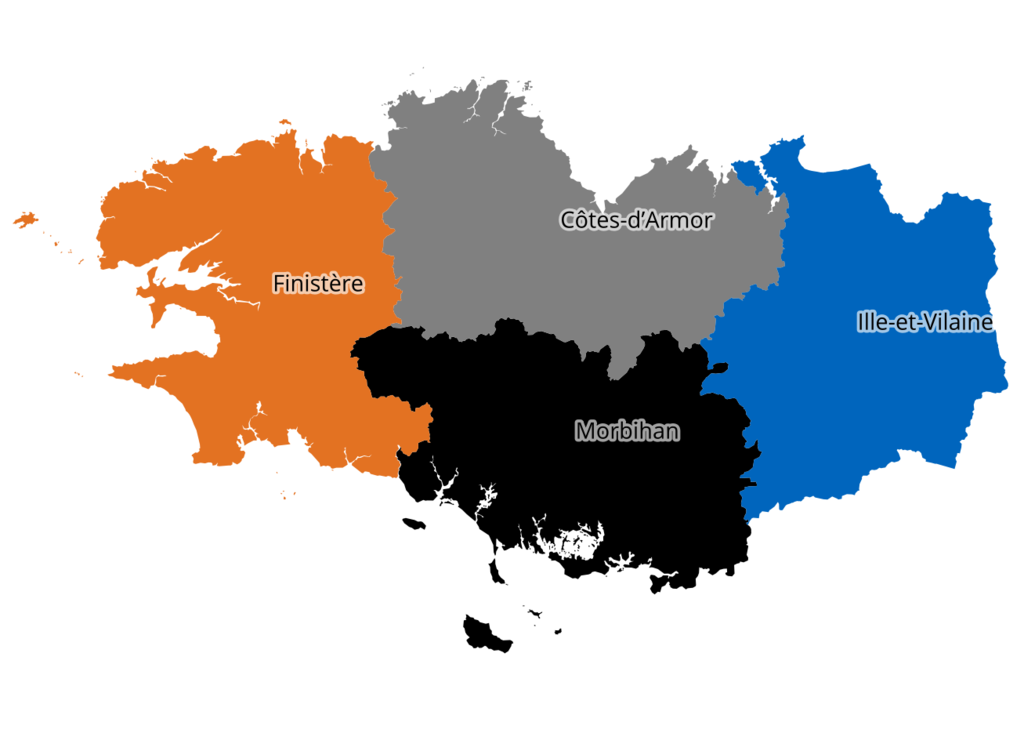
\includegraphics[width=3cm]{images/map/regions}
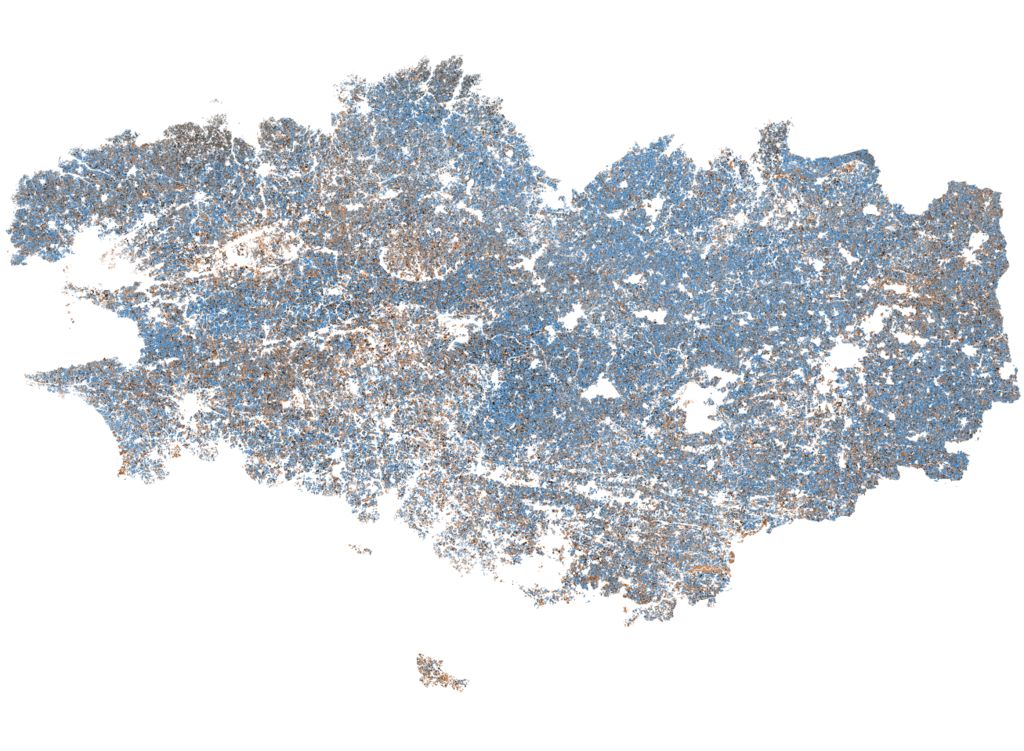
\includegraphics[width=3cm]{images/map/breizh}
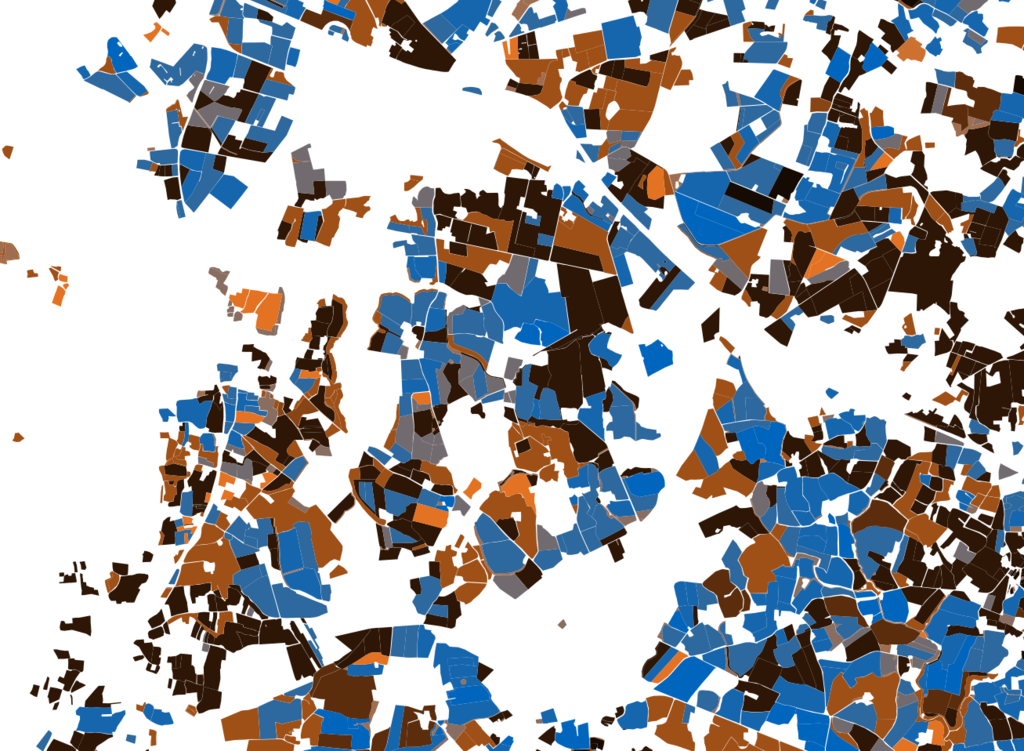
\includegraphics[width=3cm]{images/map/parcels}

\vspace{1em}

%\tikzsetnextfilename{example}

\newcommand{\dataexample}[1]{
	
	
	


\begin{tikzpicture}
	
	\tikzstyle{annot} = [font=\tiny\sffamily, text=tumblue]
	\tikzstyle{point} = [thin, tumbluelight, shorten >= .25em, shorten <= .25em]
	
	% from /home/marc/projects/EV2019/images/example/tstop.txt
	\def\tstopv{0.6285714285714286}
	\def\class{winter barley}
	
	\begin{groupplot}[
	group style={
		group name=my plots,
		group size=1 by 1,
		columns=1,
		xlabels at=edge bottom,
		xticklabels at=edge bottom,
		vertical sep=1em,
	},
	date coordinates in=x,
	date ZERO=2017-01-01,
	xmin=2017-01-01,
	xmax=2017-12-31,
	ylabel near ticks,
	ylabel style={font=\sffamily\small, rotate=-90},
	width=\textwidth,
	height=3cm,
	axis x line=bottom,
	axis y line=left,
%	enlarge x limits=0.01,
	xtick={2017-01-01,2017-05-01,2017-08-01,2017-12-01},
	xticklabels={January,April,August,December},
	ymajorgrids,
    ymax=10000
	]
	
\nextgroupplot[thin,
%	smooth=1pt,
no marks,  
ylabel={},
draw opacity=.8,
%		tension=0.001,
legend columns=2,
%y tick label style={rotate=90},
legend style={at={(.5,1)},anchor=south, line width=1pt, fill=tumblue!10}
]

\addplot[b1color] table [x=doa, y=B1, col sep=comma, forget plot] {#1};
\addplot[b9color] table [x=doa, y=B9, col sep=comma, forget plot] {#1};
\addplot[b10color] table [x=doa, y=B10, col sep=comma] {#1};

\addplot[b11color] table [x=doa, y=B11, col sep=comma, forget plot] {#1};
\addplot[b12color] table [x=doa, y=B12, col sep=comma] {#1};

\addplot[b5color] table [x=doa, y=B5, col sep=comma, forget plot] {#1};
\addplot[b6color] table [x=doa, y=B6, col sep=comma, forget plot] {#1};
\addplot[b7color] table [x=doa, y=B7, col sep=comma, forget plot] {#1};
\addplot[b8color] table [x=doa, y=B8, col sep=comma, forget plot] {#1};
\addplot[b8Acolor] table [x=doa, y=B8A, col sep=comma] {#1};

\addplot[b2color] table [x=doa, y=B2, col sep=comma, forget plot] {#1};
\addplot[b3color] table [x=doa, y=B3, col sep=comma, forget plot] {#1};
\addplot[b4color] table [x=doa, y=B4, col sep=comma] {#1};
	
%	\draw [red, very thick, ->] ([xshift=5em]plt.north west) -- ([xshift=5em]plt.south west) node [midway, rotate=90, fill=white, yshift=2pt] {faster} ;
%	\node(glab) at (10em,0.5) {ground (signal)};
	
%	\sample{images/example/3685593.csv}
%	
%	\sample{images/example/6053223.csv}
%	\draw[fill=white, draw=none, opacity=.5] (axis cs:\tstopv,0) rectangle (axis cs:1,1.1);
	
%	\node[annot](cllab) at (axis cs:.2,1.3) {clouds (noise)};
%	\draw[point] (cllab) -- (axis cs:.13,.7);
%	\draw[point] (cllab) -- (axis cs:.25,.7);
%	\draw[point] (cllab) -- (axis cs:.53,1);
%	\draw[point] (cllab) -- (axis cs:.45,.85);
%	
%	\node[annot](glab) at (axis cs:.8,1.3) {ground (signal)};
%	\draw[point] (glab) -- (axis cs:.38,.3);
%	\draw[point] (glab) -- (axis cs:.21,.3);
%	\draw[point] (glab) -- (axis cs:.7,.3);
%	
%	\draw (axis cs:\tstopv,0) -- (axis cs:\tstopv,1) node[above]{$\tstop$};
%	
%	
%	
%	\legend{3 atmospheric, 2 short-wave infrared, 5 near infrared, 3 visible bands}
%	
		\end{groupplot}
	
	\end{tikzpicture}
	
}
\begin{columns}
	\column{.5\textwidth}
	
	\textbf{corn grain and silage}
	\dataexample{images/breizhcrops/example/6139251.csv}
	
	\column{.5\textwidth}
	
	\textbf{temporary meadows}
	\dataexample{images/breizhcrops/example/3685593.csv}
	
\end{columns}

\vspace{1em}

\Large
580k samples of Time Series $\M{X}$ and labels $\V{y}$. \Large \url{https://github.com/TUM-LMF/BreizhCrops}

\end{frame}


\begin{frame}
\frametitle{Challenges and Impact}

\Large

\begin{columns}[t]

\column{.5\textwidth}

\visible<1->{
	\textbf{Impact}
	\vspace{1em}
	
	\begin{description}[itemsep=.5em]
		\item large scale \textbf{real-world dataset}
		\item effectively \textbf{unlimited data} (spatially and temporally)
		\item \textbf{assessing generalization} over large regions
		\item potential for further \textbf{vegetation characteristics} (drought indicator, early classification, crop yield)
	\end{description}
}

\column{.5\textwidth}

\visible<2->{
	\textbf{Challenges}
	\vspace{1em}
	
	\begin{description}[itemsep=.5em]
		\item \textbf{Imbalanced} class \textbf{labels}
		\item Classes with \textbf{similar characteristics}
		\item Non-Gaussian noise induced by \textbf{clouds}
		\item \textbf{Regional} \textbf{variations} in the class distributions
		\item \textbf{Spatial} \textbf{autocorrelation}
		\item \textbf{Irregular} temporal \textbf{sampling} distance
		\item \textbf{Variable} \textbf{sequence} length
	\end{description}
}


\end{columns}

\end{frame}


\begin{frame}
\frametitle{Multi-Layer RNN baseline}

\newcommand{\confmat}[3]{

\begin{tikzpicture}

  \def\vmax{#3}
  \def\dataindex{#2}
  
%
%  \pgfplotsset{every axis label/.append style={font=\footnotesize},tick pos=right, ylabel near ticks}
%  
%  \pgfplotsset{
%    axis line style={%
%      opacity=0 
%    }   
%  }

  \begin{groupplot}[
  	group style={
  		group size=2 by 1,
  		xlabels at=edge bottom,
  		ylabels at=edge left,
  		xticklabels at=edge bottom,
  		vertical sep=35pt,
  		group name=seq_len_plot
  	},
  	axis line style={draw=none},
  	title style={yshift=.75em,},
    width=6cm,
    height=6cm,
    enlargelimits=false,
    xtick=data,
%     ymin=1,
    xtick distance=1,
    ytick distance=1,
    colormap={example}{%
		color=(tumwhite)%color=(tumbluelight)
%		color=(tumivory)
%		color=(tumorange)
		color=(tumblue)%color=(tumbluelight)
%		color=(tumblack)
	},
    ytick=data,
    ytick align=outside,
    xtick align=outside,
%    tick style={draw=none},
    ytick pos = left,  
    tick label style = {font=\tiny\sansmath\sffamily},
    %xticklabel = {xshift=-0.75cm}
    yticklabel pos=left,
    %yticklabel near ticks,
    xlabel={\normalsize predicted},
    xlabel style={yshift=1em},
    ylabel style={yshift=-3em},
    x label style={at={(axis description cs:0.5,1)},anchor=south},
    y label style={at={(axis description cs:-0.1,.5)},anchor=south},
    ylabel={\normalsize ground truth},
%     ylabel near ticks,
%    xticklabels={},
  ]
  \nextgroupplot[
%      yticklabels={
%%      	{sugar beet},
%%      	{summer oat},
%%      	{meadow},
%%      	{rape},
%%      	%{vegetable},
%%      	{hop},
%%      	{winter spelt},
%%      	{winter triticale},
%%      	{beans},
%%      	{peas},
%%      	{potato},
%%      	{soybeans},
%%      	{asparagus},
%%      	{winter wheat},
%%      	{winter barley},
%%      	{winter rye},
%%      	{summer barley},
%%      	{maize}
%      },
%      xticklabels={
%%      	{sug.},
%%      	{s. oat},
%%      	{mead.},
%%      	{rape},
%%      	%{vegetable},
%%      	{hop},
%%      	{w. spelt},
%%      	{w. trit.},
%%      	{beans},
%%      	{peas},
%%      	{potato},
%%      	{soyb.},
%%      	{asp.},
%%      	{w. wheat},
%%      	{w. barley},
%%      	{w. rye},
%%      	{s. barley},
%%      	{maize}
%      },
     %colorbar style={title={\precisionrecall}, xshift=0cm, font=\footnotesize},
     colorbar right,
     colorbar style={
        	title={}, 
        	font=\footnotesize,
        	%at={(0,1)},
        	anchor=north west,
        	width=8pt,
        	ticklabel pos=right,
        	ticklabel style={xshift=2em},
%        	label style={yshift=-1em},
        	rounded corners=1pt
     },
  ]
  
    \addplot[
      matrix plot,
%      draw=tumwhite,
%       nodes near coords=\coordindex,
%       nodes near coords align={center},
%       nodes near coords style={font=\scriptsize},
        shader=faceted,
        faceted color=tumgraylight!20,
%       shader=faceted interp,
      mesh/cols=13,
      empty line=scanline,
      point meta=explicit,
      point meta min=0,
      point meta max=\vmax,
    ] table[meta index=\dataindex] {#1};
%   \nextgroupplot[
%       title=2017,
%       %colorbar style={title={\precisionrecall}, xshift=0cm, font=\footnotesize},
%       colorbar right,
%       colorbar style={
%       	title={a}, 
%       	font=\footnotesize,
%       	%at={(0,1)},
%       	anchor=north west,
%       	width=8pt,
%       	ticklabel pos=right,
%       	ticklabel style={xshift=1em},
%       	label style={yshift=1em},
%       	rounded corners=1pt
%       },
%       yticklabels={},
%     xticklabels={
%           	{sug.},
%           	{s. oat},
%           	{mead.},
%           	{rape},
%           	%{vegetable},
%           	{hop},
%           	{w. spelt},
%           	{w. trit.},
%           	{beans},
%           	{peas},
%           	{potato},
%           	{soyb.},
%           	{asp.},
%           	{w. wheat},
%           	{w. barley},
%           	{w. rye},
%           	{s. barley},
%           	{maize}
%     },
%       ]
%    
%    \addplot[
%    matrix plot,
%%    draw=tumwhite,
%    ,   
%    %       nodes near coords=\coordindex,
%    %       nodes near coords align={center},
%    %       nodes near coords style={font=\scriptsize},
%    shader=faceted,
%    faceted color=tumgraylight,
%    %       shader=faceted interp,
%    mesh/cols=17,
%    empty line=scanline,
%    point meta=explicit,
%    point meta min=0,
%    point meta max=\vmax,
%    ] table[meta index=\dataindex] {images/confmat/formatted_grucm2017.csv};
    
  \end{groupplot}
\end{tikzpicture}
}

\begin{columns}

\column{.5\textwidth}
\textbf{Precision}

\confmat{images/data/BreizhCrops_rnn/npy/confmat_flat.csv}{3}{1}

\column{.5\textwidth}
\textbf{Recall}

\confmat{images/data/BreizhCrops_rnn/npy/confmat_flat.csv}{4}{1}

\end{columns}

\end{frame}

\begin{frame}
\frametitle{Transformer baseline}

\newcommand{\confmat}[3]{

\begin{tikzpicture}

  \def\vmax{#3}
  \def\dataindex{#2}
  
%
%  \pgfplotsset{every axis label/.append style={font=\footnotesize},tick pos=right, ylabel near ticks}
%  
%  \pgfplotsset{
%    axis line style={%
%      opacity=0 
%    }   
%  }

  \begin{groupplot}[
  	group style={
  		group size=2 by 1,
  		xlabels at=edge bottom,
  		ylabels at=edge left,
  		xticklabels at=edge bottom,
  		vertical sep=35pt,
  		group name=seq_len_plot
  	},
  	axis line style={draw=none},
  	title style={yshift=.75em,},
    width=6cm,
    height=6cm,
    enlargelimits=false,
    xtick=data,
%     ymin=1,
    xtick distance=1,
    ytick distance=1,
    colormap={example}{%
		color=(tumwhite)%color=(tumbluelight)
%		color=(tumivory)
%		color=(tumorange)
		color=(tumblue)%color=(tumbluelight)
%		color=(tumblack)
	},
    ytick=data,
    ytick align=outside,
    xtick align=outside,
%    tick style={draw=none},
    ytick pos = left,  
    tick label style = {font=\tiny\sansmath\sffamily},
    %xticklabel = {xshift=-0.75cm}
    yticklabel pos=left,
    %yticklabel near ticks,
    xlabel={\normalsize predicted},
    xlabel style={yshift=1em},
    ylabel style={yshift=-3em},
    x label style={at={(axis description cs:0.5,1)},anchor=south},
    y label style={at={(axis description cs:-0.1,.5)},anchor=south},
    ylabel={\normalsize ground truth},
%     ylabel near ticks,
%    xticklabels={},
  ]
  \nextgroupplot[
%      yticklabels={
%%      	{sugar beet},
%%      	{summer oat},
%%      	{meadow},
%%      	{rape},
%%      	%{vegetable},
%%      	{hop},
%%      	{winter spelt},
%%      	{winter triticale},
%%      	{beans},
%%      	{peas},
%%      	{potato},
%%      	{soybeans},
%%      	{asparagus},
%%      	{winter wheat},
%%      	{winter barley},
%%      	{winter rye},
%%      	{summer barley},
%%      	{maize}
%      },
%      xticklabels={
%%      	{sug.},
%%      	{s. oat},
%%      	{mead.},
%%      	{rape},
%%      	%{vegetable},
%%      	{hop},
%%      	{w. spelt},
%%      	{w. trit.},
%%      	{beans},
%%      	{peas},
%%      	{potato},
%%      	{soyb.},
%%      	{asp.},
%%      	{w. wheat},
%%      	{w. barley},
%%      	{w. rye},
%%      	{s. barley},
%%      	{maize}
%      },
     %colorbar style={title={\precisionrecall}, xshift=0cm, font=\footnotesize},
     colorbar right,
     colorbar style={
        	title={}, 
        	font=\footnotesize,
        	%at={(0,1)},
        	anchor=north west,
        	width=8pt,
        	ticklabel pos=right,
        	ticklabel style={xshift=2em},
%        	label style={yshift=-1em},
        	rounded corners=1pt
     },
  ]
  
    \addplot[
      matrix plot,
%      draw=tumwhite,
%       nodes near coords=\coordindex,
%       nodes near coords align={center},
%       nodes near coords style={font=\scriptsize},
        shader=faceted,
        faceted color=tumgraylight!20,
%       shader=faceted interp,
      mesh/cols=13,
      empty line=scanline,
      point meta=explicit,
      point meta min=0,
      point meta max=\vmax,
    ] table[meta index=\dataindex] {#1};
%   \nextgroupplot[
%       title=2017,
%       %colorbar style={title={\precisionrecall}, xshift=0cm, font=\footnotesize},
%       colorbar right,
%       colorbar style={
%       	title={a}, 
%       	font=\footnotesize,
%       	%at={(0,1)},
%       	anchor=north west,
%       	width=8pt,
%       	ticklabel pos=right,
%       	ticklabel style={xshift=1em},
%       	label style={yshift=1em},
%       	rounded corners=1pt
%       },
%       yticklabels={},
%     xticklabels={
%           	{sug.},
%           	{s. oat},
%           	{mead.},
%           	{rape},
%           	%{vegetable},
%           	{hop},
%           	{w. spelt},
%           	{w. trit.},
%           	{beans},
%           	{peas},
%           	{potato},
%           	{soyb.},
%           	{asp.},
%           	{w. wheat},
%           	{w. barley},
%           	{w. rye},
%           	{s. barley},
%           	{maize}
%     },
%       ]
%    
%    \addplot[
%    matrix plot,
%%    draw=tumwhite,
%    ,   
%    %       nodes near coords=\coordindex,
%    %       nodes near coords align={center},
%    %       nodes near coords style={font=\scriptsize},
%    shader=faceted,
%    faceted color=tumgraylight,
%    %       shader=faceted interp,
%    mesh/cols=17,
%    empty line=scanline,
%    point meta=explicit,
%    point meta min=0,
%    point meta max=\vmax,
%    ] table[meta index=\dataindex] {images/confmat/formatted_grucm2017.csv};
    
  \end{groupplot}
\end{tikzpicture}
}

\begin{columns}

\column{.5\textwidth}
\confmat{images/data/BreizhCrops_transformer/npy/confmat_flat.csv}{3}{1}

\column{.5\textwidth}
\confmat{images/data/BreizhCrops_transformer/npy/confmat_flat.csv}{4}{1}

\end{columns}

\end{frame}


\begin{frame}
\frametitle{Going Big...}

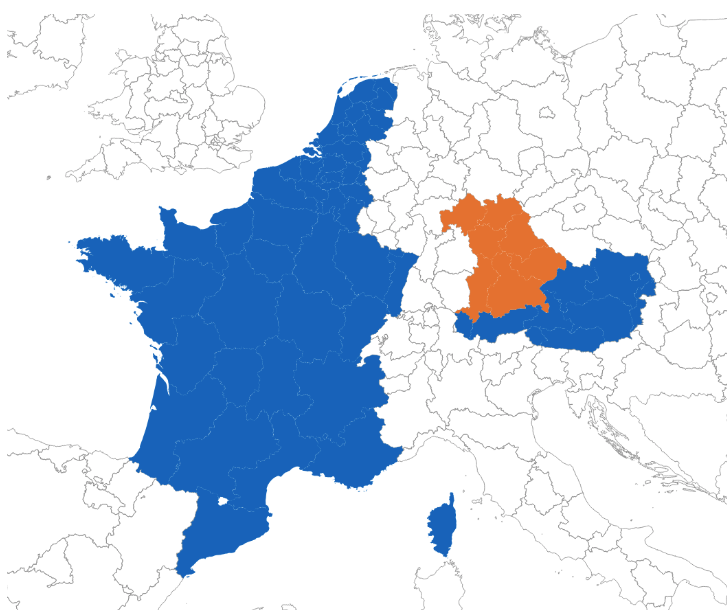
\includegraphics[width=5cm]{images/EuroCrops}
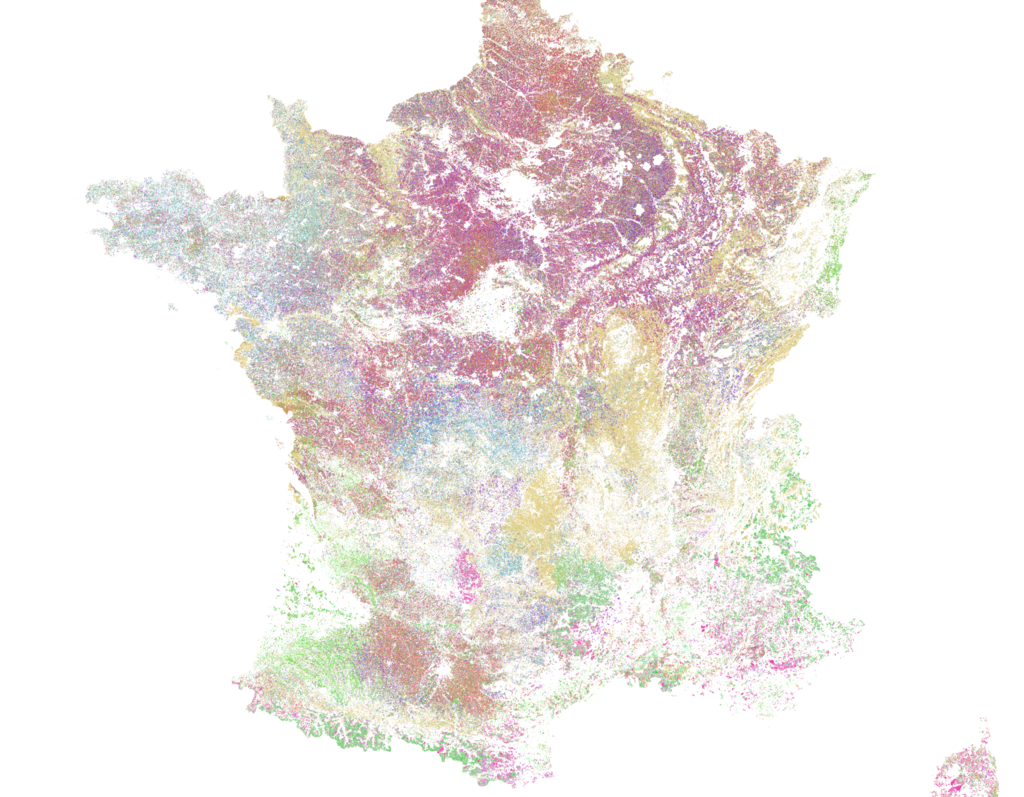
\includegraphics[width=5cm]{images/France}
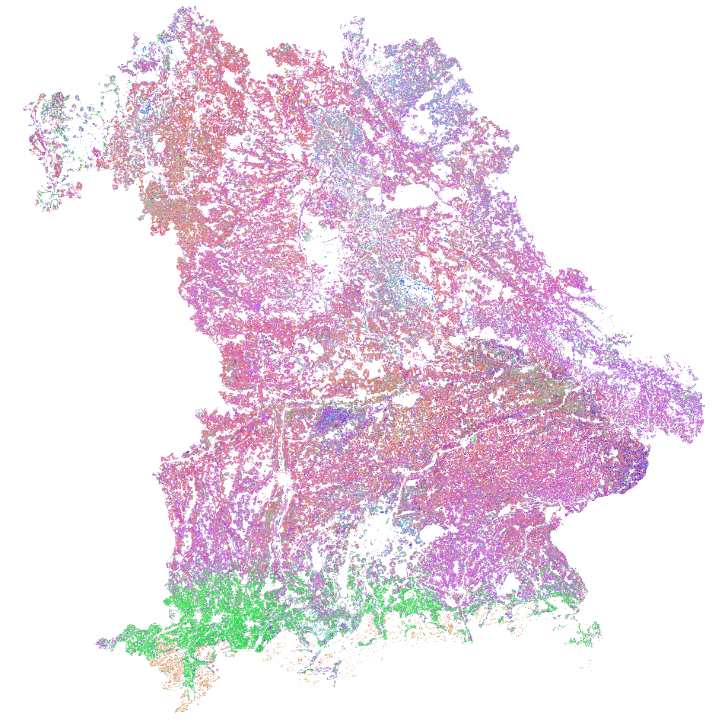
\includegraphics[width=4cm]{images/Bavaria}

\end{frame}

\begin{frame}
\frametitle{Supported by Google Research Credits}


\includegraphics[width=.3\textwidth]{images/google_research_credits}

\includegraphics[width=.3\textwidth]{images/google}

\includegraphics[width=.2\textwidth]{images/earth-engine-logo}
%
\includegraphics[width=3cm]{images/250px-Google-Cloud-Storage-Logo}
%
\includegraphics[width=3cm]{images/Google_Compute_Engine_logo}
%
\includegraphics[width=3cm]{images/google_cloud_sql}


\end{frame}


\end{document}



